\documentclass{resume}

\usepackage[none]{hyphenat}
% \usepackage{breakurl}
\begin{document}

\fontfamily{ppl}\selectfont


\noindent
\begin{tabularx}{\linewidth}{@{}m{0.8\textwidth} m{0.2\textwidth}@{}}
{
    \Large{Artem Batalov} \newline
    \small{
        \clink{
            \href{mailto:a@batalov.me}{a@batalov.me} \textbf{·} 
            {\fontdimen2\font=0.75ex +7 906 959-50-30} 
            \textbf{·} 
            \href{https://batalov.me}{batalov.me}
        } \newline
        Innopolis, Russia
    }
} & 
{
    \hfill
    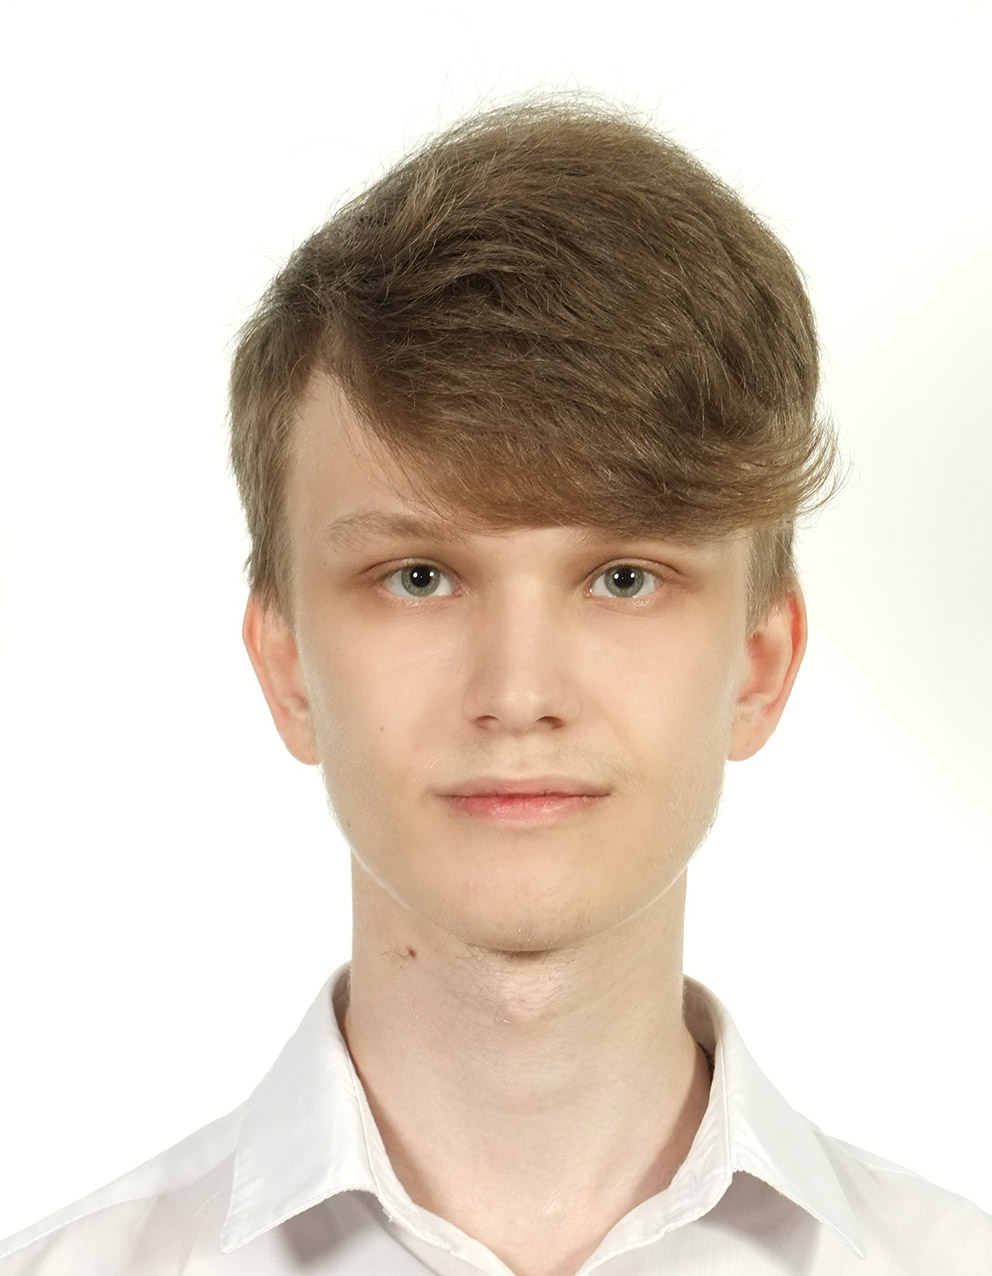
\includegraphics[width=2.8cm]{images/photo.jpg}
}
\end{tabularx}


\begin{center}
\begin{tabularx}{\linewidth}{@{}*{2}{X}@{}}
% left side %
{
    \csection{EDUCATION}{\small
        \begin{itemize}
            \item \frcontent{Bachelor Student in Computer Science}{Innopolis University}{}{2020 - now}
        \end{itemize}
    }
    \csection{EXPERIENCE}{\small
        \begin{itemize}
            \item \frcontent{Municipal institution centre by career planning}{Full-stack developer − Tomsk, Russia}{Co-designer and co-implementor of scheduling system and timetable visualization (\href{http://rasp.cpc.tomsk.ru}{rasp.cpc.tomsk.ru}).}{June 2019 to December 2019}
            
            \item \frcontent{SberDevices}{Intern − Innopolis, Russia}{Front-End developer of SmartApp for alarms and timers.\newline
            React, Typescript}{April 2021 to July 2021}
            
            \item \frcontent{SberDevices}{Junior Python Developer − Innopolis, Russia}{Working on Intent Recognizer system, and Framework for making speaking assistants}{August 2021 to now}
        \end{itemize}
    }
    \csection{PROJECTS}{\small
        \begin{itemize}
            \item \frcontent{Drone Swarm \newline \clink{\href{https://github.com/bart02/DroneSwarm}{[github.com/bart02/DroneSwarm]}}}{Software for making the drone show with drones controlled by Raspberry Pi and PX4 flight.}{}{Python}
            
            \item \frcontent{Human Express \newline \clink{\href{https://github.com/Tennessium/HUEX}{[github.com/Tennessium/HUEX]}}}{A system that monitors the movement of a group of drones in real time.}{}{Python, Web}
        \end{itemize}
    }
    % \csection{HOBBIES \& INTERESTS}{\small
    %     \vspace{0.32cm}
    %     \begin{tabularx}{\linewidth}{@{}*{4}{>{\centering\arraybackslash}X}@{}}
    %         {\centering
    %         
\includegraphics[width=0.8cm]{images/userexperience.png}
    %         } &
    %         {\centering
    %         
\includegraphics[width=0.8cm]{images/lamp.png}
    %         } & 
    %         {\centering
    %         
\includegraphics[width=0.8cm]{images/healthcare.png}
    %         } &
    %         {\centering
    %         
\includegraphics[width=0.8cm]{images/cauldron.png}
    %         } \\
    %         {\footnotesize Drones \& Robotics} & {\footnotesize Machine Learning} & {\footnotesize Technical creativity} & {\footnotesize Open Source}
    %     \end{tabularx}
    % }
} 
% end left side %
& 
% right side %
{
    \csection{SKILLS}{\small
        \begin{itemize}
            \item \textbf{Hard Skills} \newline
            {\footnotesize Python, C++, PHP, Docker; \newline
            \textbf{Front-end}: HTML, CSS, JS, Typescript, Vue, React}
            
            \item \textbf{Soft Skills} \newline
            {\footnotesize Time-Management, Agile, Scrum}
            
            \item \textbf{Language Skills} \newline
            {\footnotesize \textbf{Russian}: Native Speaker; \newline
            \textbf{English}: Upper-Intermediate}
        \end{itemize}
    }
    \csection{ACHIEVEMENTS}{\small
        \begin{itemize}
            \item \frcontent{Video-to-features service for media \newline \textit{(Digital Breakthrough - 2021, Final)} \newline \clink{\href{https://gitlab.com/znayut-shto-delayut}{[gitlab.com/znayut-shto-delayut]}}}{A service to help media in creating recommender system that gets features from a video reportage.}{\textbf{I place}}{Python, Web}
            
            \item \frcontent{Machine learning models evaluation web-service \textit{(Digital Breakthrough - 2020)} \newline \clink{\href{https://github.com/SyrexMinus/model_comparison_service}{[github.com/SyrexMinus/model\_\newline comparison\_service]}}}{A web service for visually comparing the performance of machine learning models.}{\textbf{II place}}{Python, Web}
            
            \item \frcontent{LifeStyle Assistant \textit{(SberCode - 2021)} \newline \clink{\href{https://gitlab.com/lifestyleassistant}{[gitlab.com/lifestyleassistant]}}}{A life-style SmartApp for Sber Salute application.}{\textbf{I place}}{Python, Web}
            
            \item \frcontent{Easy To Fly \textit{(CopterHack - 2021)} \newline \clink{\href{https://github.com/bart02/EasyToFly}{[github.com/bart02/EasyToFly]}}}{Software and hardware for make drone control easily.}{\textbf{II place}}{ROS, Python, Web}
        \end{itemize}
    }
    % \csection{AWARDS \& RECOGNITION}{\small
    %     \begin{itemize}
    %         \item \frcontent{Nadav Shoham RoboTraffic Competition}{\textbf{I place} in Careful Driving nonimation, \newline
    %         \textbf{I place} in Project nonimation, \newline
    %         \textbf{III place} in Racing nomination}{}{2019}
            
    %         \item \frcontent{"Big Cahllenges" project program}{Double winner}{}{2018, 2019}
    %     \end{itemize}
    % }

    % \csection{OTHER HIGHLIGHTS}{\small
    %     \begin{itemize}
    %         \item {\footnotesize Gave talk on \textit{Achieving Rapid Response Times in Large Online Services} at Berkeley AMPLab Cloud.}
    %         \item {\footnotesize Led several teams across infrastructure, founded \textit{Google Brain} and was involved in hiring process.}
    %     \end{itemize}
    % }
}
\end{tabularx}
\end{center}
\end{document}